\section{Avoided crossings}

The first step required to reach two-qubits gates is the avoided crossing experiment~\cite{Silveri2015, Sun2020}.
The objective here is to find, approximately, the flux and frequency where the interaction will happen.

In particular, since we are considering the iSWAP, we want to find the point in the flux-frequency space, where we can have a jump of states between $\ket{01}$ and $\ket{10}$.

We are considering to have two flux-controllable qubits already calibrated (at the single qubit level) so we are supposing to have already studied the flux dependency of those, but let's repeat some information.
Both qubits have a dependency between frequency and the flux passing through their SQUID.
They are characterized by a certain sweetspot, namely a certain flux value that moves the qubit to a frequency that is the maximum frequency reachable.
The application of less or more flux will reduce the frequency of the qubits.

Note that we now want to control both qubits at the same time and a flux applied at one will probably change also the other qubit. It's critical to take this in consideration in the research for the sweetspots.

Anyway, considering one qubit (A) at the sweetspot and the second qubit (B), that has a higher frequency at the sweetspot, swept in bias, we can obtain a plot similar to the one in \cref{fig:crossings}.

\begin{figure}[ht]
    \centering
    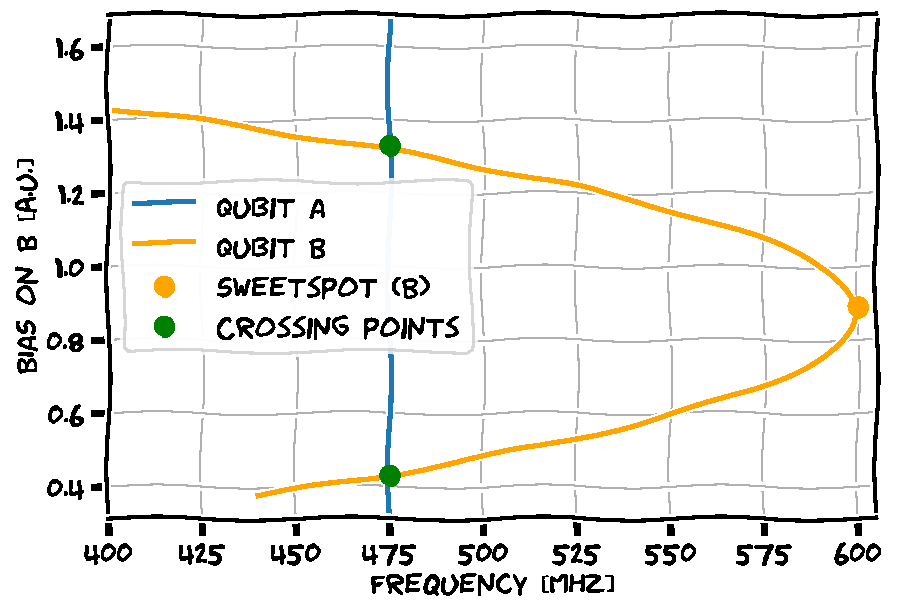
\includegraphics[width=8cm]{Two-qubits calibration/Figures/crossings.pdf}
    \caption{Possible behaviour of two qubits flux dependence.}
    \label{fig:crossings}
\end{figure}

Note that in \cref{fig:crossings} the lines are the ones drawn by the peaks in qubit spectroscopies that describes the transition $\ket 0 \leftrightarrow \ket 1$.

Note also that, if we define the two-qubits state as $\ket A \otimes \ket B = \ket{AB}$, we can identify the orange curve in the plot as the one of the $\ket{00} \leftrightarrow \ket{01}$ transition and the blue one as the $\ket{00} \leftrightarrow \ket{10}$ transition.
So at the green points we have precisely the condition required for the iSWAP and, to reach it, it seems that is just needed to apply two contemporary flux pulses at two qubits (with an amplitude computed from the distance from the sweetspot).

What actually is happening at the crossing points however, is an hybridization of the two states that can be solved analytically or just seen directly by zooming in the plot presented. 
See for example \cref{fig:avoided_crossing} (note that the axes are swapped).
\begin{figure}[ht]
    \centering
    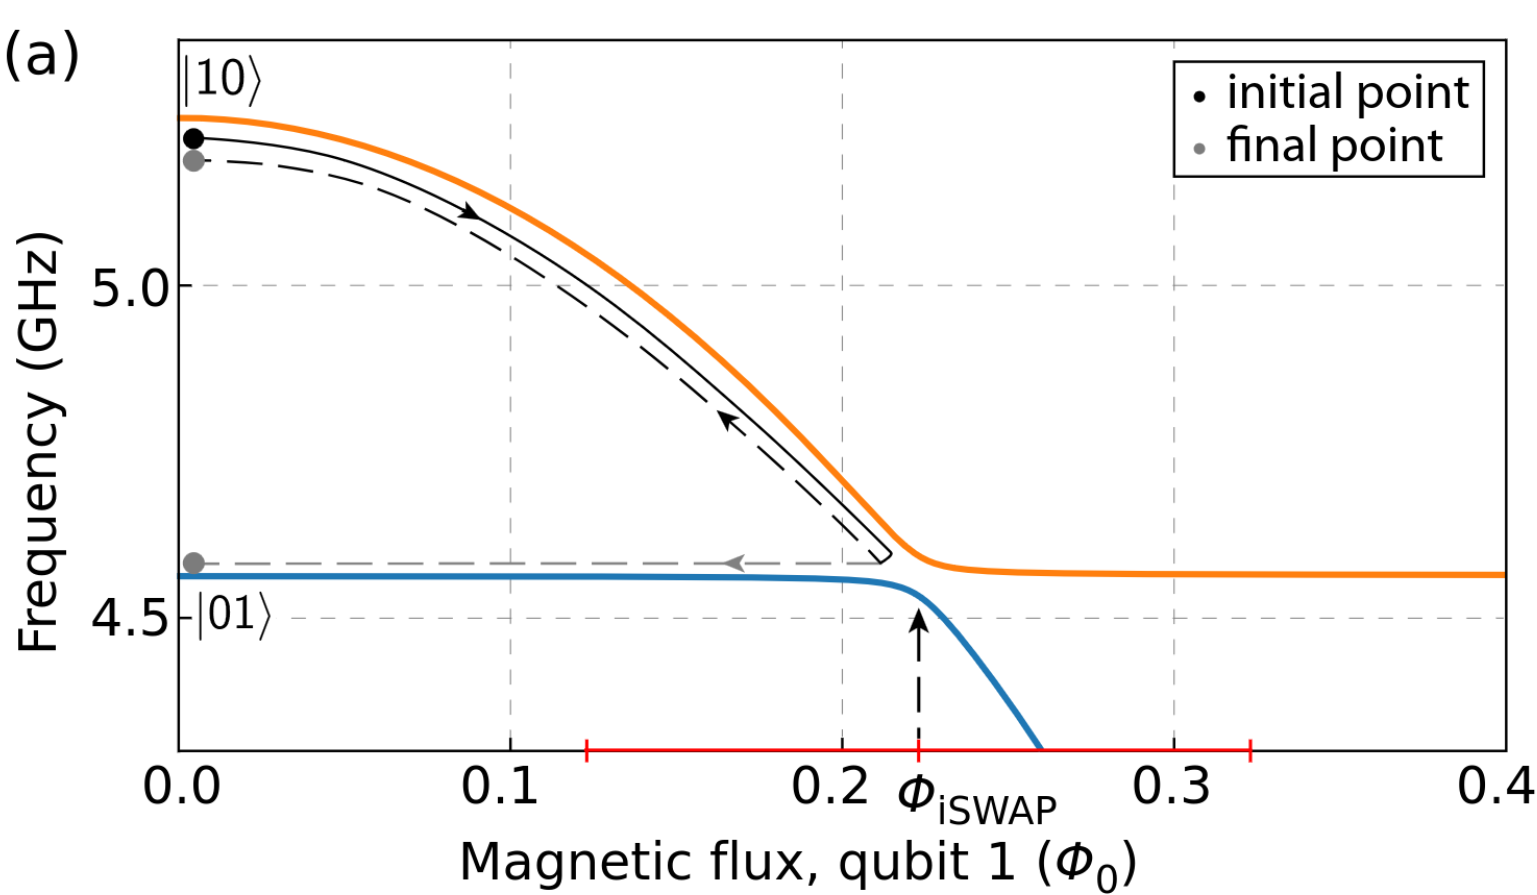
\includegraphics[width=8cm]{Two-qubits calibration/Figures/avoided_crossing.png}
    \caption{Avoided crossing.}
    \label{fig:avoided_crossing}
\end{figure}

In \cref{fig:avoided_crossing} it's defined also an initial and final state, that will be used for the iSWAP.

Finding the avoided crossings is the first step for two-qubits gates characterization.
After that, we know how much flux is needed to move the higher frequency qubit to the interaction point and we have proved (through avoided crossing) that an interaction is indeed present (but we still need to calibrate it).

Note that there are always two interaction points, but this are usually at different flux absolute values, so it's preferred to use the lower one (although the interaction would happen equally.

Note also that we now saw the avoided crossings for the iSWAP, but for the CZ the experiment is similar.
For the CZ we look for the interaction $\ket{02} \leftrightarrow \ket {20}$.
To see the second level transition frequency, it is sufficient to perform a qubit spectroscopy with more amplitude so that, just before the $\ket 0 \leftrightarrow \ket 1$ transition peak, also the $\frac{\ket 0 \leftrightarrow \ket 2}{2}$ can appear (divided by two because usually two combined photons can give those high energies).

A larger scan in frequencies can give us \cref{fig:avoided_crossing2}.
\begin{figure}[ht]
    \centering
    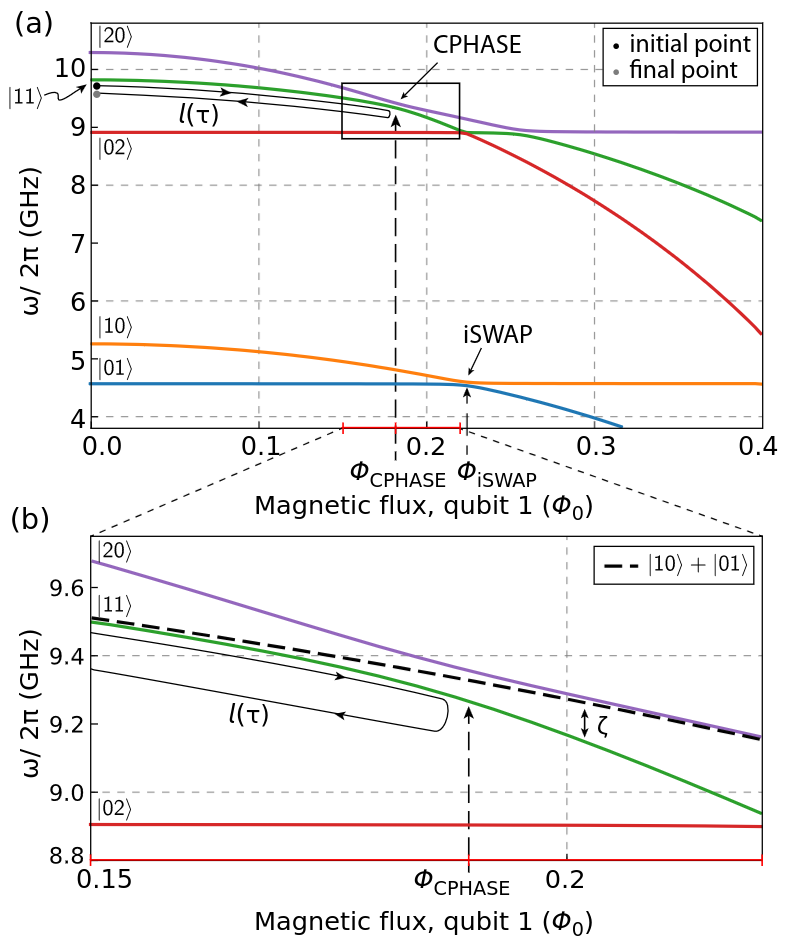
\includegraphics[width=8cm]{Two-qubits calibration/Figures/crossing_cz_iswap.png}
    \caption{Avoided crossing for CZ and iSWAP.}
    \label{fig:avoided_crossing2}
\end{figure}

In \cref{fig:crossings_large} are shown the results of a scan large both in flux and frequency.
The 4 horizontal lines are a low resolution visualization of the 4 avoided crossings (2 for CZ and 2 for iSWAP) with the inner two being the ones for CZ and the outer two of iSWAP.

\begin{figure}[ht]
    \centering
    \makebox[\textwidth][c]{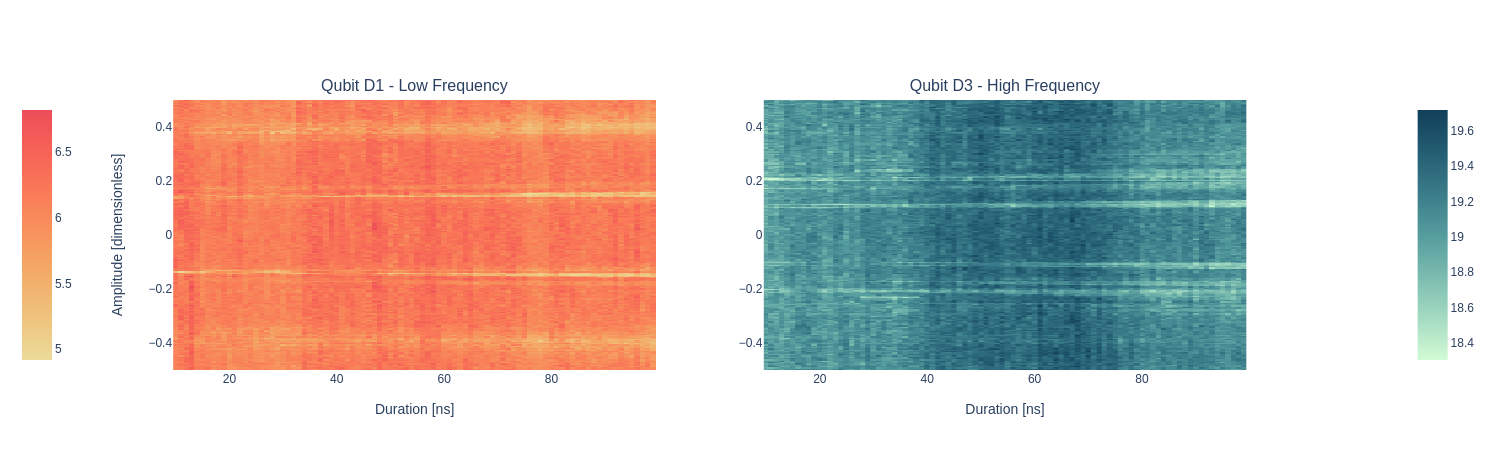
\includegraphics[width=1.3\textwidth]{Two-qubits calibration/Figures/large_chevron.png}}
    \caption{Large scan where all the 4 interaction biases are visible.}
    \label{fig:crossings_large}
\end{figure}

In \cref{fig:avoided_crossing_qblox} a zoom in on one of the iSWAP crossing points show the states hybridization and the avoided crossing phenomenon.

\begin{figure}[htbp]
    \centering
    \makebox[\textwidth][c]{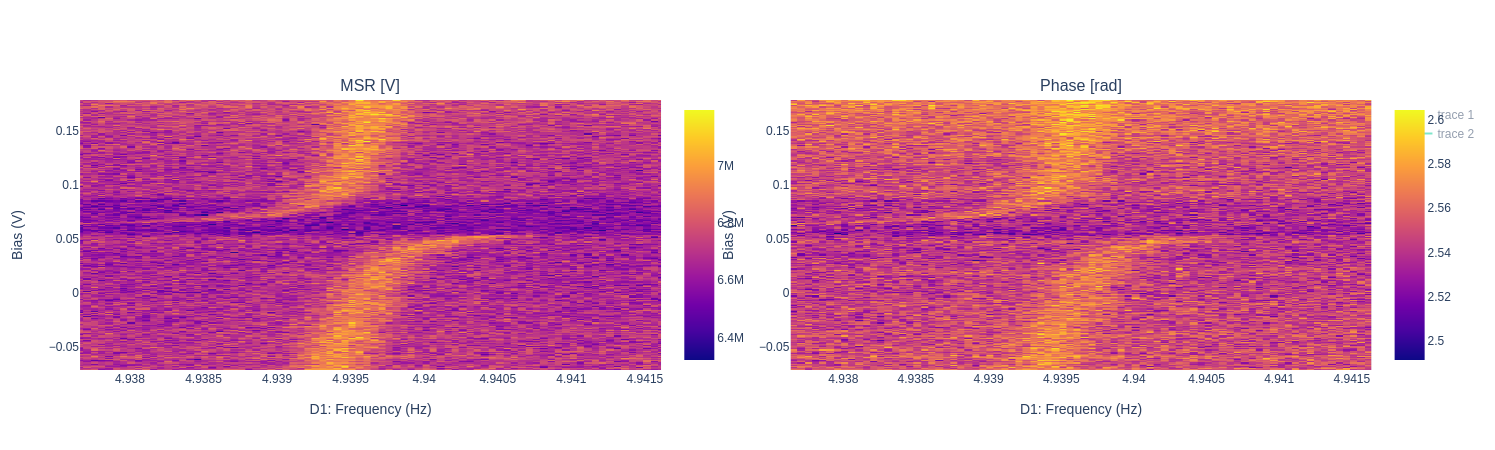
\includegraphics[width=1.3\textwidth]{Two-qubits calibration/Figures/my_avoided_crossing.png}}
    \caption{Zoom in on an avoided crossing (iSWAP). The bias is applied only to the high frequency qubit, while the lower is left at the sweetspot. Measuring the low-frequency qubit gives the avoided crossing.}
    \label{fig:avoided_crossing_qblox}
\end{figure}





